\section{Ser to NS}
\label{appendix:delta-req-resp-examples}

\begin{figure}[!htbp]
	\centering
	%–––– Network system diagram ––––
	% 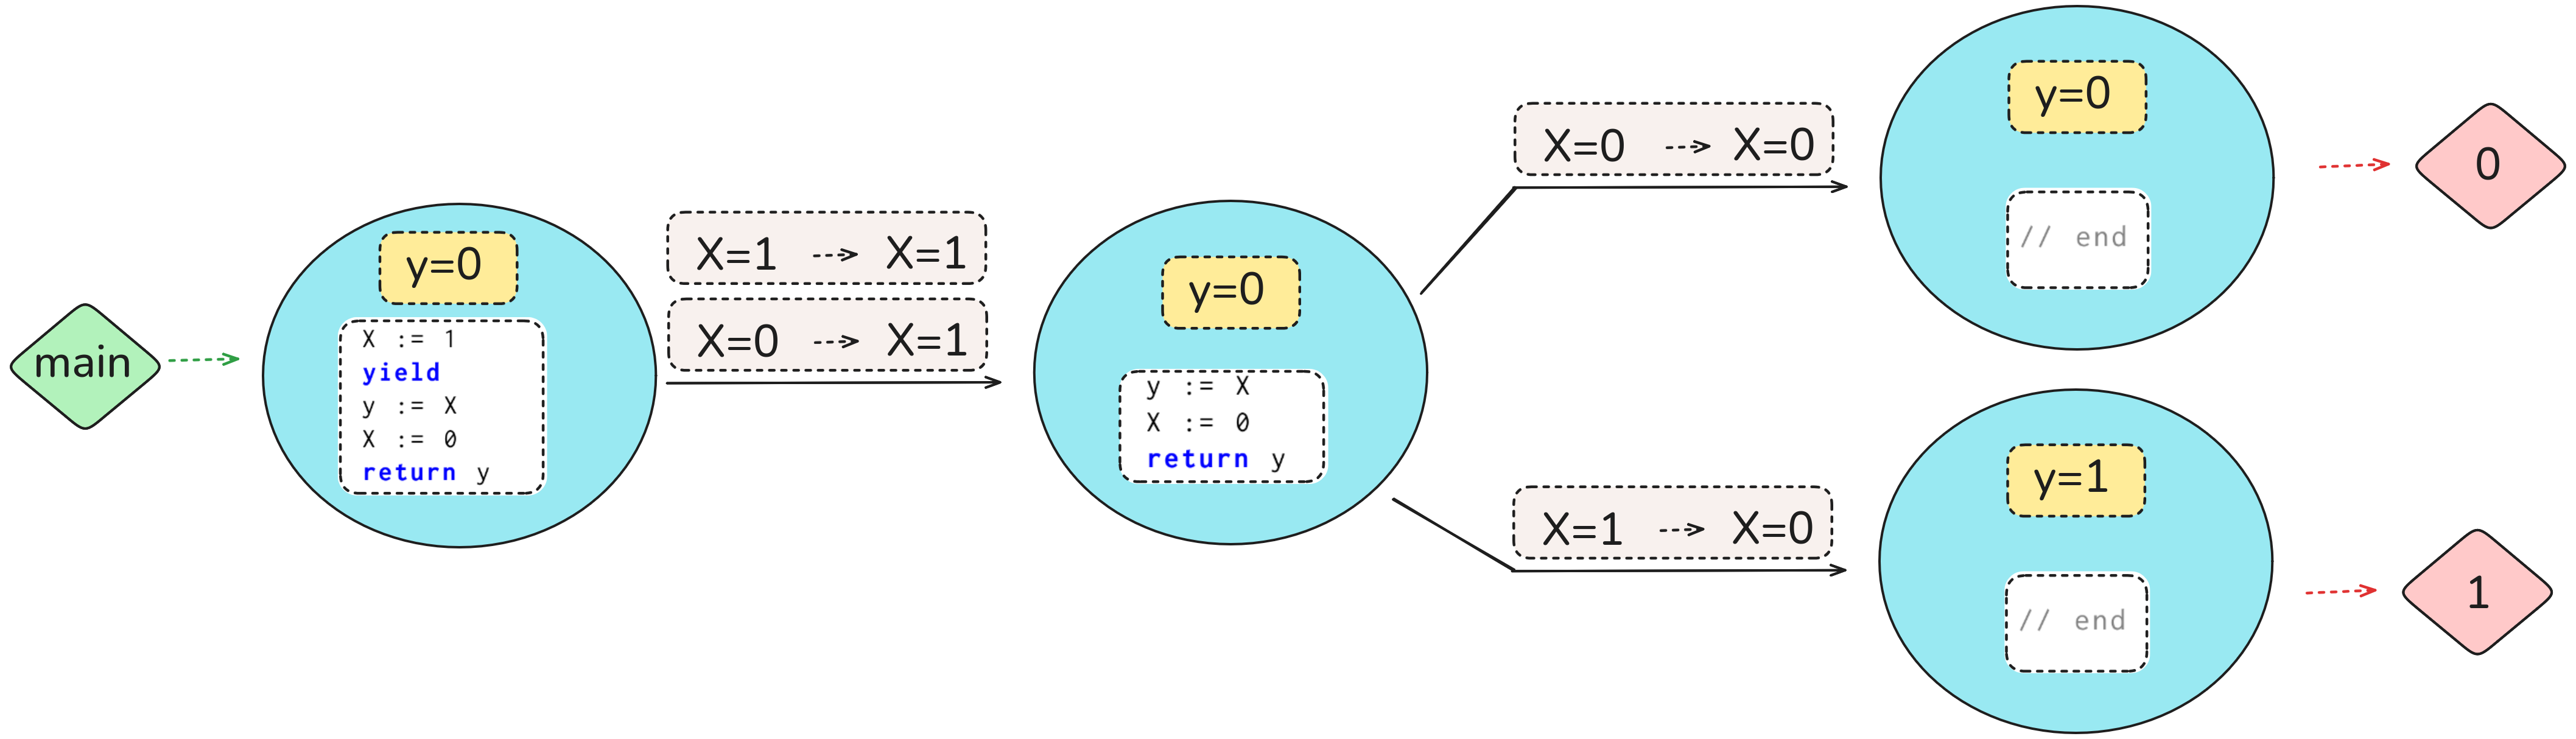
\includegraphics[width=\textwidth]{plots/code_2_NS.png}\\[1ex]
	
	%–––– req, resp, and δ definitions ––––
	\[
	\begin{array}{@{}r@{\;}l}
		req \coloneq & 
		\big\{
		\big[
		\begin{array}{c c c}
			\begin{tikzpicture}[baseline=(textnode.base)]
				\node[
				draw=black,
				line width=0.8pt,
				fill=ForestGreen!20,
				text=black,
				diamond,
				aspect=2,
				inner sep=2pt,
				scale=0.7
				] (textnode) {\texttt{main}};
			\end{tikzpicture}
			&\!\!\rightarrow\!\!&
			\begin{array}{c}
				\begin{tikzpicture}[baseline=(ybox.base)]
					\node[
					draw=black,
					line width=0.8pt,
					fill=brightyellow,
					text=black,
					rectangle,
					rounded corners=1pt,
					inner sep=2pt
					] (ybox) {\texttt{y=0}};
				\end{tikzpicture}\vspace{-2pt}
				\\
				\begin{minipage}{0.20\linewidth}
					\begin{lstlisting}[language=CustomPseudoCode,numbers=none,basicstyle=\tiny\ttfamily]
						X := 1 
						yield 
						y := X
						X := 0
						return y
					\end{lstlisting}
				\end{minipage}
			\end{array}
		\end{array}
		\big]
		\big\}
		\\[2em]
		resp \coloneq &
		\big\{
		\big[
		\begin{array}{c c c}
			\begin{array}{c}
				\begin{tikzpicture}[baseline=(ybox.base)]
					\node[
					draw=black,
					line width=0.8pt,
					fill=brightyellow,
					text=black,
					rectangle,
					rounded corners=1pt,
					inner sep=2pt
					] (ybox) {\texttt{y=0}};
				\end{tikzpicture}\vspace{-2pt}
				\\
				\begin{minipage}{0.11\linewidth}
					\begin{lstlisting}[language=CustomPseudoCode,numbers=none,basicstyle=\tiny\ttfamily]
						// end
					\end{lstlisting}
				\end{minipage}
			\end{array}
			&\!\!\rightarrow\!\!&
			\begin{tikzpicture}[baseline=(textnode.base),scale=0.7]
				\node[
				draw=black,
				line width=0.8pt,
				fill=RedViolet!20,
				text=black,
				diamond,
				aspect=2,
				inner sep=2pt,
				font=\small
				] (textnode) {\texttt{0}};
			\end{tikzpicture}
		\end{array}
		\big]\,{},
		\big[
		\begin{array}{c c c}
			\begin{array}{c}
				\begin{tikzpicture}[baseline=(ybox.base)]
					\node[
					draw=black,
					line width=0.8pt,
					fill=brightyellow,
					text=black,
					rectangle,
					rounded corners=1pt,
					inner sep=2pt
					] (ybox) {\texttt{y=1}};
				\end{tikzpicture}\vspace{-2pt}
				\\
				\begin{minipage}{0.11\linewidth}
					\begin{lstlisting}[language=CustomPseudoCode,numbers=none,basicstyle=\tiny\ttfamily]
						// end
					\end{lstlisting}
				\end{minipage}
			\end{array}
			&\!\!\rightarrow\!\!&
			\begin{tikzpicture}[baseline=(textnode.base),scale=0.7]
				\node[
				draw=black,
				line width=0.8pt,
				fill=RedViolet!20,
				text=black,
				diamond,
				aspect=2,
				inner sep=2pt,
				font=\small
				] (textnode) {\texttt{1}};
			\end{tikzpicture}
		\end{array}
		\big]
		\big\}
		\\[2em]
		\delta \coloneq & 
		\big\{\big[(
		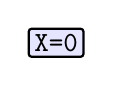
\begin{tikzpicture}[baseline=(ybox.base)]
			\node[
			draw=black,
			line width=0.8pt,
			fill=blue!10,
			text=black,
			rectangle,
			rounded corners=1pt,
			inner sep=2pt
			] (ybox) {\texttt{X=0}};
		\end{tikzpicture}\,{},
		\begin{array}{c}
			\begin{tikzpicture}[baseline=(ybox.base)]
				\node[
				draw=black,
				line width=0.8pt,
				fill=brightyellow,
				text=black,
				rectangle,
				rounded corners=1pt,
				inner sep=2pt
				] (ybox) {\texttt{y=0}};
			\end{tikzpicture}\vspace{-2pt}
			\\
			\begin{minipage}{0.14\linewidth}
				\begin{lstlisting}[language=CustomPseudoCode,numbers=none,basicstyle=\tiny\ttfamily]
					X := 1
					yield
					y := X
					X := 0
					return y
				\end{lstlisting}
			\end{minipage}
		\end{array}
		)
		\;\rightarrow\;
		(
		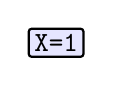
\begin{tikzpicture}[baseline=(ybox.base)]
			\node[
			draw=black,
			line width=0.8pt,
			fill=blue!10,
			text=black,
			rectangle,
			rounded corners=1pt,
			inner sep=2pt
			] (ybox) {\texttt{X=1}};
		\end{tikzpicture}\,{},
		\begin{array}{c}
			\begin{tikzpicture}[baseline=(ybox.base)]
				\node[
				draw=black,
				line width=0.8pt,
				fill=brightyellow,
				text=black,
				rectangle,
				rounded corners=1pt,
				inner sep=2pt
				] (ybox) {\texttt{y=0}};
			\end{tikzpicture}\vspace{-2pt}
			\\
			\begin{minipage}{0.14\linewidth}
				\begin{lstlisting}[language=CustomPseudoCode,numbers=none,basicstyle=\tiny\ttfamily]
					y := X
					X := 0
					return y
				\end{lstlisting}
			\end{minipage}
		\end{array}
		)
		\big],
		\\[0.5em]
		& \phantom{\big\{}
		\big[(
		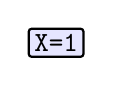
\begin{tikzpicture}[baseline=(ybox.base)]
			\node[
			draw=black,
			line width=0.8pt,
			fill=blue!10,
			text=black,
			rectangle,
			rounded corners=1pt,
			inner sep=2pt
			] (ybox) {\texttt{X=1}};
		\end{tikzpicture}\,{},
		\begin{array}{c}
			\begin{tikzpicture}[baseline=(ybox.base)]
				\node[
				draw=black,
				line width=0.8pt,
				fill=brightyellow,
				text=black,
				rectangle,
				rounded corners=1pt,
				inner sep=2pt
				] (ybox) {\texttt{y=0}};
			\end{tikzpicture}\vspace{-2pt}
			\\
			\begin{minipage}{0.14\linewidth}
				\begin{lstlisting}[language=CustomPseudoCode,numbers=none,basicstyle=\tiny\ttfamily]
					y := X
					X := 0
					return y
				\end{lstlisting}
			\end{minipage}
		\end{array}
		)
		\;\rightarrow\;
		(
		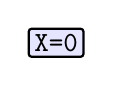
\begin{tikzpicture}[baseline=(ybox.base)]
			\node[
			draw=black,
			line width=0.8pt,
			fill=blue!10,
			text=black,
			rectangle,
			rounded corners=1pt,
			inner sep=2pt
			] (ybox) {\texttt{X=0}};
		\end{tikzpicture}\,{},
		\begin{array}{c}
			\begin{tikzpicture}[baseline=(ybox.base)]
				\node[
				draw=black,
				line width=0.8pt,
				fill=brightyellow,
				text=black,
				rectangle,
				rounded corners=1pt,
				inner sep=2pt
				] (ybox) {\texttt{y=1}};
			\end{tikzpicture}
			\vspace{-2pt}
			\\
			\begin{minipage}{0.11\linewidth}
				\begin{lstlisting}[language=CustomPseudoCode,numbers=none,basicstyle=\tiny\ttfamily]
					// end
				\end{lstlisting}
			\end{minipage}
		\end{array}
		)
		\big],
		\ldots
		\big\}
	\end{array}
	\]
	\caption{The \(\delta\) transition function, and the \(req\) and \(res\) mappings for the program in Listing~\ref{lst:MotivatingExample2NonSer}.}
	\label{fig:code2ExampleNSSecondPart}
\end{figure}
